\chapter{Design}

\section{Overall System Design}

\subsection{Short description of the main parts of the system}
\begin{itemize}
	\item Stock Database System
	\begin{itemize}
		\item User Interface
		\item Adding a new product
		\item Editing a product
		\item Viewing information about Stock
	\end{itemize}
\end{itemize}

User Interface:
\begin{itemize}
	\item Upon launching the program, the user will be presented with an option of 4 buttons. The first button says "Add new Product", the second "Edit a product", the third "View all products" and the fourth "Exit"
	\item After selecting the "Add new Product" option, the user is taken to a new user interface where they can enter in information about a new product to the database.
	\item Clicking the "Edit a product" option will present the user with a new user interface where they are able to delete a product from the database.
	\item Clicking the "View all  products" option wil present the user with a new user interface where they can search for a product from the database.
	\item Clicking the "Exit" option will close the program.
\end{itemize}
Adding a new product:
\begin{itemize}
	\item After clicking the "Add new Product" button on the main menu, the user is presented with a new user interface.
	\item On this new interface, the user is presented with a series of boxes with labels indicating the type of information that should be entered.
	\item When all the information has been entered, the user will be able to click the submit button at the bottom of the page, which will add the information as a new record in the database.
\end{itemize}

Editing a product: 
\begin{itemize}
	\item After clicking the "Edit a product" button, the user will be taken to a new user interface.
	\item On this new interface, the user is given an option of choosing a product from the database, and editing its information.
\end{itemize}


Viewing information about stock
\begin{itemize}
	\item After clicking the "View all products" button on the main menu, the user is taken to a new user interface.
	\item On the new interface, the user is presented with a table of all of the products and their information in one table.
\end{itemize}
\subsection{System flowcharts showing an overview of the complete system}
\begin{figure}[H]
	\centering
	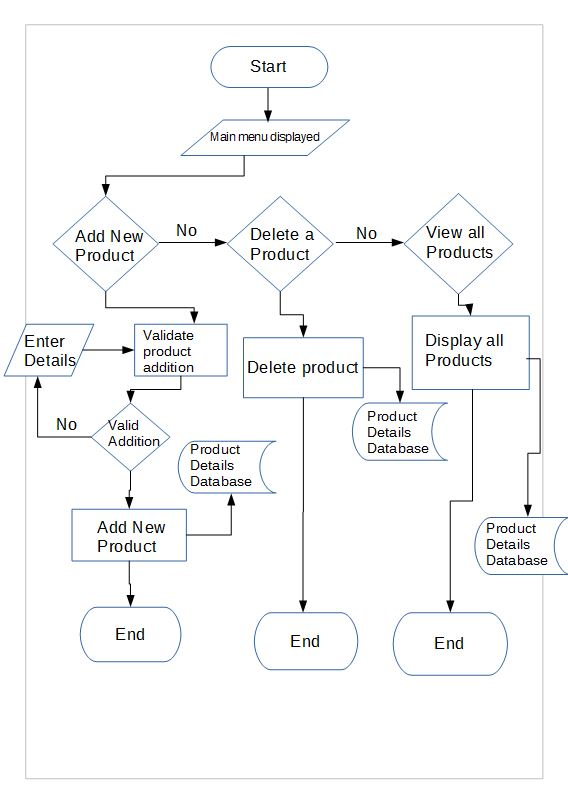
\includegraphics[width= 10cm, height = 15.5cm]{Design/images/design_flow_charts.JPG}
	\caption {System Flowchart} \label{fig:system_flow_chart}
\end{figure}
\section{User Interface Designs}

\section{Hardware Specification}
The system will be run on a laptop/desktop running Windows 10 and with a 1920x1080 resolution and a 16:10 aspect ratio screen. This is important as I will have to ensure that my program is the correct size for the size of the screen. A keyboard will be required, in order to input information into the database. A mouse will also be required in order to navigate around the program and to select options from the main menu. A display will be used for the output of the of the program. The programs data will be held on the internal hard drive.
\section{Program Structure}

\subsection{Top-down design structure charts}

\begin{figure}[H]
	\centering
	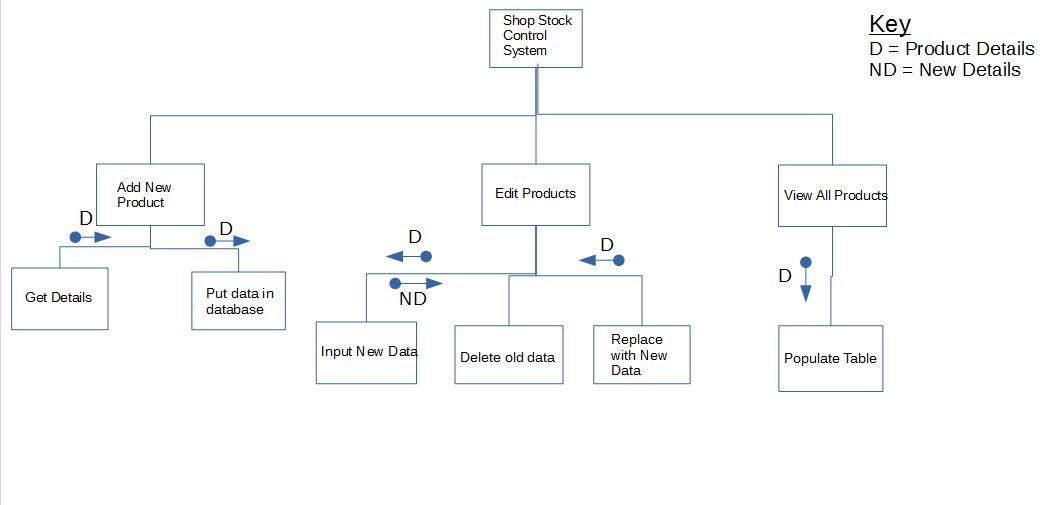
\includegraphics[width= 20cm, height = 15.5cm]{Design/images/Hierarchy_Chart.JPG}
	\caption {System Design Structure Chart} \label{fig:system_design_structure_chart}
\end{figure}

\subsection{Algorithms in pseudo-code for each data transformation process}

\subsection{Object Diagrams}

\subsection{Class Definitions}

\section{Prototyping}

\begin{figure}[H]
	\centering
	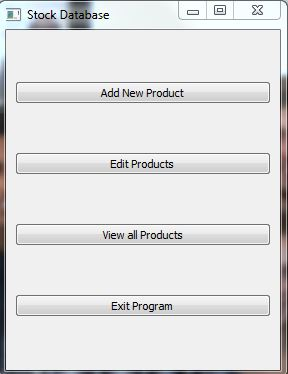
\includegraphics[width= 8cm, height = 10.5cm]{Design/images/menu_prototype.JPG}
	\caption {Main Menu Protype} \label{fig:main_menu_prototype}
\end{figure}

\begin{figure}[H]
	\centering
	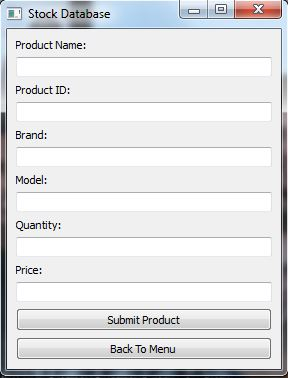
\includegraphics[width= 8cm, height = 10.5cm]{Design/images/new_product_prototype.JPG}
	\caption {Add New Product Prototype} \label{fig:add_new_product_prototype}
\end{figure}

\begin{figure}[H]
	\centering
	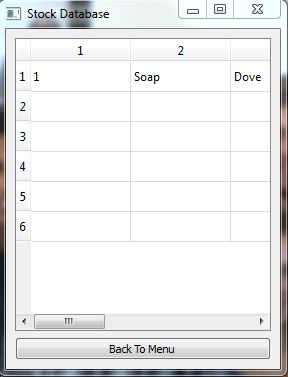
\includegraphics[width= 8cm, height = 10.5cm]{Design/images/database_prototype.JPG}
	\caption {View Database Prototype} \label{fig:view_database_prototype}
\end{figure}
\section{Definition of Data Requirements}

\subsection{Identification of all data input items}

\subsection{Identification of all data output items}

\subsection{Explanation of how data output items are generated}

\subsection{Data Dictionary}

\subsection{Identification of appropriate storage media}

\section{Database Design}

\subsection{Normalisation}

\subsubsection{ER Diagrams}

\subsubsection{Entity Descriptions}

\subsubsection{1NF to 3NF}

\subsection{SQL Queries}

\section{Security and Integrity of the System and Data}

\subsection{Security and Integrity of Data}

\subsection{System Security}

\section{Validation}

\section{Testing}

\begin{landscape}
\subsection{Outline Plan}

\begin{center}
    \begin{tabular}{|p{2cm}|p{5cm}|p{5cm}|p{4cm}|}
        \hline
        \textbf{Test Series} & \textbf{Purpose of Test Series} & \textbf{Testing Strategy} & \textbf{Strategy Rationale}\\ \hline
        Example & Example & Example & Example \\ \hline
    \end{tabular}
\end{center}

\subsection{Detailed Plan}

\begin{center}
    \begin{longtable}{|p{1.5cm}|p{2.5cm}|p{2.5cm}|p{2cm}|p{2cm}|p{2cm}|p{2cm}|p{2cm}|}
        \hline
        \textbf{Test Series} & \textbf{Purpose of Test} & \textbf{Test Description} & \textbf{Test Data} & \textbf{Test Data Type (Normal/ Erroneous/ Boundary)} & \textbf{Expected Result} & \textbf{Actual Result} & \textbf{Evidence}\\ \hline
        Example & Example & Example & Example & Example & Example & Example & Example \\ \hline
    \end{longtable}
\end{center}
\end{landscape}